\documentclass[NormeDiProgetto.tex]{subfiles}

\begin{document}
	
	\chapter{Processi organizzativi}
	
	\section{Comunicazione}
	\subsection{Comunicazioni interne}
	\subsection{Comunicazioni esterne}
	
	\section{Riunioni}
	\subsection{Verbale di riunione}
	\subsection{Riunioni interne}
	\subsection{Riunioni esterne}
	
	\section{Ruoli di progetto}
	\subsection{Responsabile di progetto}
	\subsection{Amministratore}
	\subsection{Analista}
	\subsection{Progettista}
	\subsection{Programmatore}
	\subsection{Verificatore}
	
	\section{Formazione del personale}
	La formazione del personale è da realizzarsi in maniera autonoma. I membri del gruppo 353 sono tenuti a studiare individialmente le tecnologie che verranno utilizzate nel corso del progetto. \'{E} possibile che i membri dele gruppo realizzino, in piena libertà, delle guide a carattere informale e relative ad un singolo argomento, allo scopo di facilitare la formazione ai restanti componenti del gruppo. La documentazione di riferimento, oltre che al materiale già citato nella sottosezione \emph{Riferimenti Informativi}, comprende:\\
	\begin{itemize}
		\item Per l'utilizzo di \LaTeX: \url{https://www.latex-project.org/} \\
		\item Per l'utilizzo di GitHub: \url{https://github.com/}\\
		\item Per l'utilizzo di React: \url{https://reactjs.org/}\\
		\item Per l'utilizzo di Redux: \url{https://redux.js.org/}\\
		\item Per l'utilizzo di Ethereum: \url{https://www.ethereum.org/}\\
		\item Per l'utilizzo di Metamask, \url{https://metamask.io/}\\ 
		\item Per l'utilizzo di Solidity: \url{https://solidity.readthedocs.io/en/develop/}\\
	\end{itemize}
	Il versionamento dei prodotti servirà anche per apprendere dall'operato
	altrui, in modo da integrare le conoscenze personali migliorando la qualità e
	l'effcienza delle attività.
	\section{Ambiente di lavoro}
	\subsection{Coordinamento}
\subparagraph{Versionamento:} Per quel che riguarda il versionamento si è scelto di utilizzare Git, in quanto molto flessibile e già utilizzato, o quantomeno conosciuto, da tutti i membri del gruppo 353, nonchè in quanto consigliatoci dal Referente.\\
		\'{E} stato scelto di preferire, come servizo di hosting, GitHub piuttosto che BitBucket, a causa della non gratuità di quest'ultimo. GitHub inoltre presenta un utile bot per l'integrazione con il servizio di collabroazione aziendale \emph{Slack}.
\subparagraph{Pianificazione:} Per quanto riguarda la pianificazione, la scelta del gruppo 353 è ricaduta sul Asana, strumento per la creazione e l'assegnazione di task con data di inizio e fine per la pianificazione personale del lavoro da svolgere.
\subparagraph{Standups:} Per incentivare la continuità nel tempo dello sviluppo della commessa, si è scelto di utilizzare Standup Alice, un bot per \emph{Slack} per la realizzazione giornaliera di standups, permettendo al gruppo di seguire costantemente l'operato degli altri componenti e di confrontarsi nel caso sorgano dubbi o domande.
\subparagraph{Altri strumenti:}
		\begin{itemize}
			\item \textbf{Google Drive} \'{E} stato scelto per la condivisione veloce di le come
			guide, documentazioni, riferimenti utili e documenti informali tramite
			Google Docs. Google Docs permette la creazione di documenti
			maneggevoli quando è necessaria una modica da parte di molti membri
			del gruppo (ad esempio nella fase di approvazione degli scheletri dei
			documenti); in questo Google Docs si rivela estremamente 
			essibile,
			visualizzando in tempo reale le modiche apportate al documento,
			permettendo inoltre di aggiungere commenti al testo.
			\item \textbf{Google Calendar} \'{E} stato scelto per la gestione degli eventi ed
			impegni del gruppo, come riunioni interne, revisioni od incontri con il committente. Fornisce
			inoltre un \Glossario{Bot} integrabile con \Glossario{Slack}.
		\end{itemize}
	\subsection{Documentazione}
	\subparagraph{\LaTeX:} Per quanto riguarda la stesura della documentazione, si è deciso di
		utilizzare \LaTeX. \\
		\'{E}	stato scelto questo linguaggio di \Glossario{markup}, nonostante
		non sempre sia di immediata comprensione, per le sue potenzialità quando
		si tratta di riferimenti all'interno del documento, tabelle, numerazioni,
		note, organizzazione delle pagine, creazione di template. inoltre
		la possibilità di creare comandi personalizzati, caratteristica utile nella
		stesura della documentazione prodotta nel corso del progetto. Di fronte a
		queste caratteristiche così positive, altre soluzioni possibili (come utilizzare
		LibreOffice o Google Docs) sono state immediatamente scartate.
	\subparagraph{Editor:} L'editor consigliato per scrivere la documentazione con LATEX è
		TexStudio in quanto software libero aggiornato e multi piattaforma. Esso
		permette il completamento automatico dei comandi, la codifica in UTF-8 e
		dispone di un visualizzatore PDF integrato.
	\subparagraph{Diagrammi UML:} Per la modellazione dei diagrammi UML è stato deciso di utilizzare 	\emph{UML Designer} in quanto supporta UML 1.x ed UML 2.x. Permette la modellazione dei casi d'uso, i 	diagrammi delle classi, degli oggetti, delle attività	e di sequenza.
	\subparagraph{Tracciamento:} Per il tracciamento dei requisiti e dei casi d'uso si è deciso di utilizzare \emph{Trender}, un software che permette di tener traccia delle dipendenze dei vari componenti durante lo sviluppo del progetto.
	\end{itemize}
	\subsection{Ambiente di sviluppo}
	\subparagraph{Sistemi operativi:} I membri del gruppo 353 possono operare indistintamente sui tre 		principali sitemi operativi (Windows, Mac OS X e Linux), in quanto esistono frameworks per tutte le piattaforme che sono compatibili con le librerie di sviluppo interessate.
	\subparagraph{Browsers:} \Glossario{Metamask}, il plugin che permette ad un \Glossario{browser} l'accesso alla rete \Glossario{Ethereum}, è attualmente disponibile solo per \Glossario{Google Chrome} e si rende quindi necessario l'utilizzo di quest'ultimo.
	\subsection{Ambiente di verifica}
	\subparagraph{Documentazione:} Per quanto riguarda la verifica dei documenti, TexStudio non
		ha di default il dizionario per il controllo ortografico italiano. \'{E}
		stato quindi preparato un pacchetto da scompattare all'interno della cartella
		"dictionaries" dentro la directory di installazione di TexStudio in modo da
		poter selezionare come lingua preferita l'italiano nella sezione "Controllo
		Linguistico" delle Configurazioni di TexStudio.
	\subparagraph{Codice:}
		\begin{itemize}
			\item \textbf{Analisi Statica:}
			\item \textbf{Analisi Dinamica:}
		\end{itemize}
	\subsection{Ticketing}
	Per distribuire i tasks ai vari componenti del gruppo, si è deciso di utilizzare il servizio di task manager Asana. Grazie ad una feature che permette la condivisione dei \Glossario{tasks} tra più \Glossario{boards}, è possibile avere una board dedicata alla panoramica delle marco-tasks di progetto che sono da fare. Ogni task, dopo essere stato assegnato, viene spostato in una seconda board contenente tutti i tasks attualmente fase di sviluppo. Al loro completamento vengono poi spostati in una terza board contentente i tasks da verificare. Sarà poi compito dei verificatori constatare l'effettivo completamento del task oppure la necessità di revisionare lo stesso.
	\subparagraph{Struttura di un task}
	Ogni task viene creato dal Respondabile di Progetto oppure da un membro del gruppo. Nel secondo caso è richiesta l'approvazione del task da parte della maggioranza (4) dei rimanenti componenti del gruppo.
	Ogni task è composto da un titolo significativo e \Glossario{due date} del task stesso.
	L'assegnazione del task ad uno specifico componente del gruppo può avvenire secondo due modalità:\\
	\begin{itemize}
		\item \textbf{Proattivamente:} L'assegnatario del task è già noto al momento della creazione dello stesso. In questo caso il task viene assegnato direttamente allo specifico componente del gruppo. 
		\item \textbf{Retroattivamente:} Nel caso di task a bassa priorità oppure di grandi moli di lavoro da parte di tutti i componenti del gruppo, può non essere possibile assegnare direttamente un task ad un componente del gruppo. Questi tasks possono essere auto-assegnati qualora il componente finisse in anticipo i tasks a lui già assegnati.
	\end{itemize}
	\'{E} possibile che un task cambi assegnatario durante il suo percorso di sviluppo. Tipicamente, infatti, il verificatore sarà un componente del gruppo diverso da quello che ha inizialmente preso in carico il task.
	\subparagraph{Ciclo di vita di un ticket}
	ogni task si rifà al seguente ciclo di vita a partire dalla sua creazione fino al completamento.\\
	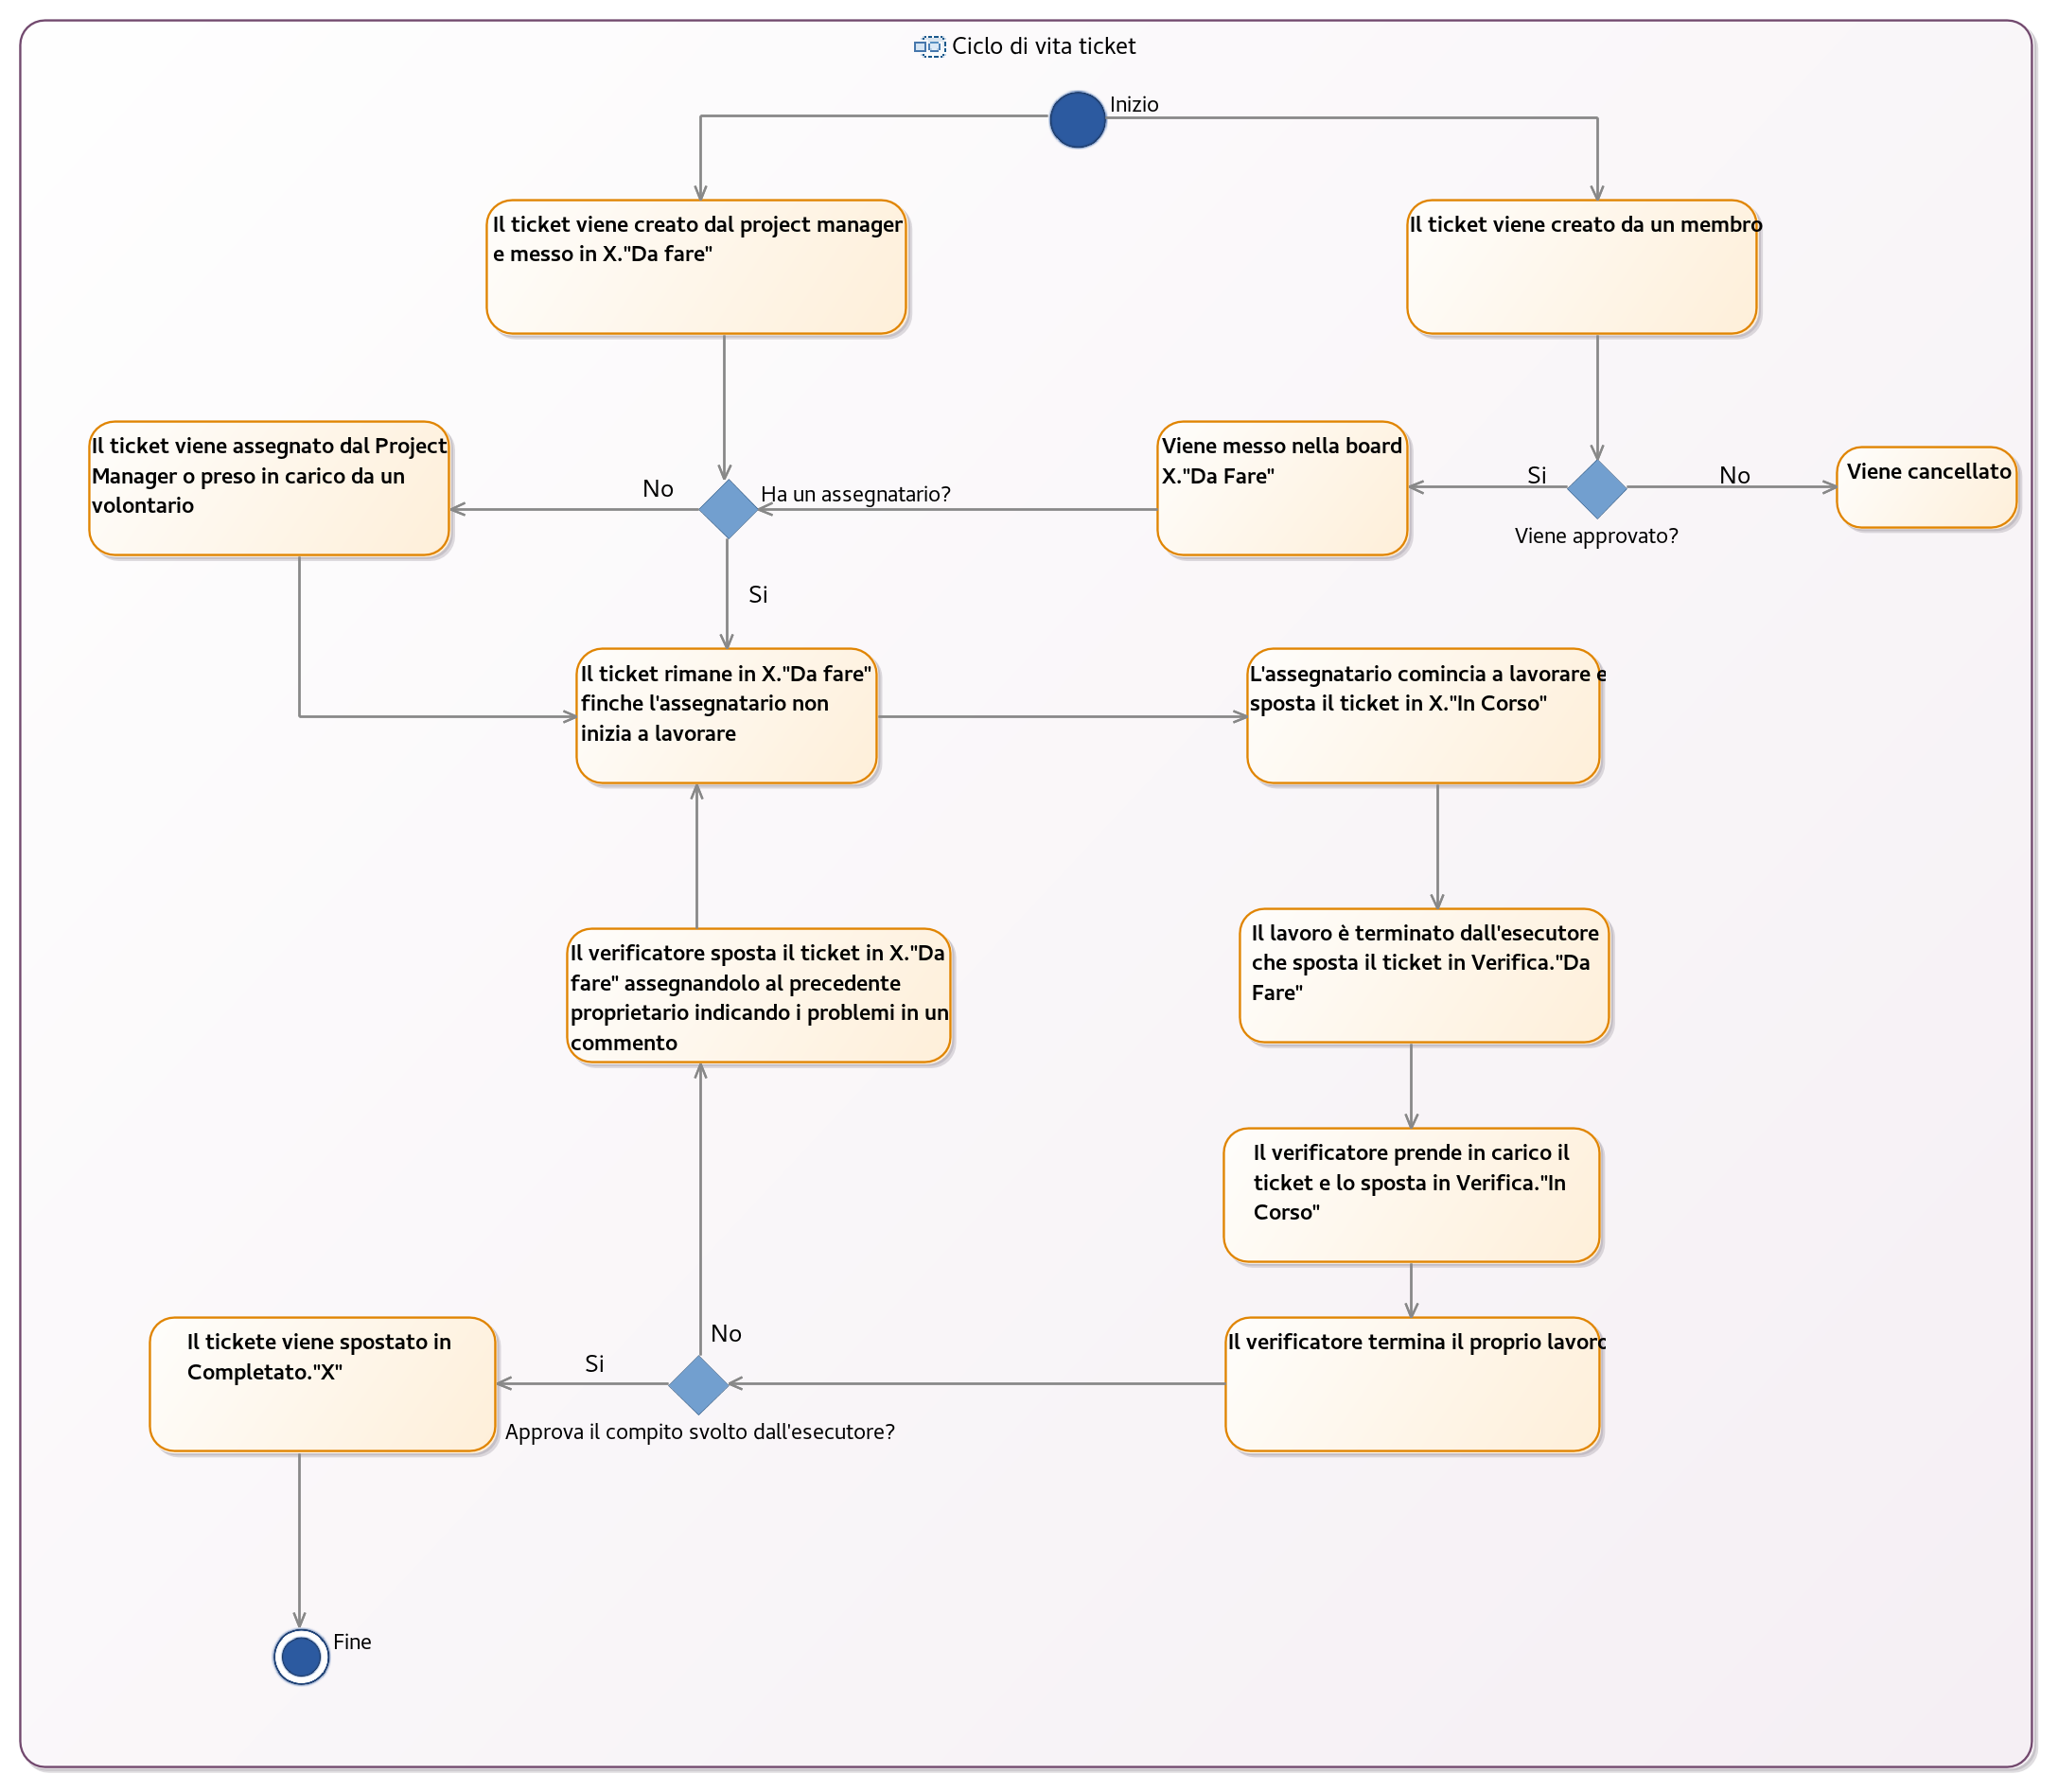
\includegraphics[scale=0.3]{../../common/images/AsanaFlow}
	\caption{Figura 4.5.5: Ciclo di vita di un ticket}
\end{document}